\chapter{Discussion}

\section{\ac{uwwls}}
Artefacts caused by unwrapping algorithm: Suggests that the algorithm is highly sensitive to strong fluctuations in \ac{oct} signal and as a result creates artefacts in these regions. Why?

\section{\ac{uwsg}}

\section{\ac{posg}}

\section{\ac{wfd}}
\begin{itemize}
	\item Strong artefacts in comparison to other images - why? Perhaps because our $OCT_{SNR}$ assumptions are breaking down sooner than we thought, and therefore not fitting accurately.
	\item Need to decide if this has something to do with OUR phantom (i.e. not actually a homogenous bulk, scatterers were not evenly distributed through as they would be in tissue), or if similar results would be seen in all images, tissue and otherwise.
	\item Another way of thinking about it would be whether these artefacts could have merit, show more contrast. However there is a need to investigate and outline more clearly what the image \textit{actually} shows. 
	\item Why did it perform so badly in the lateral image resolution? Was it a result of the region imaged (was there an optical artefact here that the lateral averaging picked up?).
\end{itemize}

\section{\ac{uwfd}}
	Looks very similar to the WLS result, which is interesting considering this method did not make use of the optical weighting. Need to investigate whether this method was only the best because of the homogenous phantom imaged, and whether or not other methods 

\section{\ac{pffd}}
\begin{itemize}
	\item Did show increase in sensitivity over all other techniques. Because the strain and lateral smoothing filter were corrected for added smoothing performed by the pre-filter, this must be due to the combination of weighted and unweighted smoothing.
 	\item Interesting to note, that took on a combination of sorts of the \ac{wfd} and \ac{uwfd} image resolutions. 
\end{itemize}

\begin{figure}
	\centering
	\begin{subfigure}{0.49\textwidth}
		\centering
		
\includegraphics[width=\textwidth]{figures/uwfd_compare.png}
	\end{subfigure}
	\begin{subfigure}{0.49\textwidth}
		\centering
		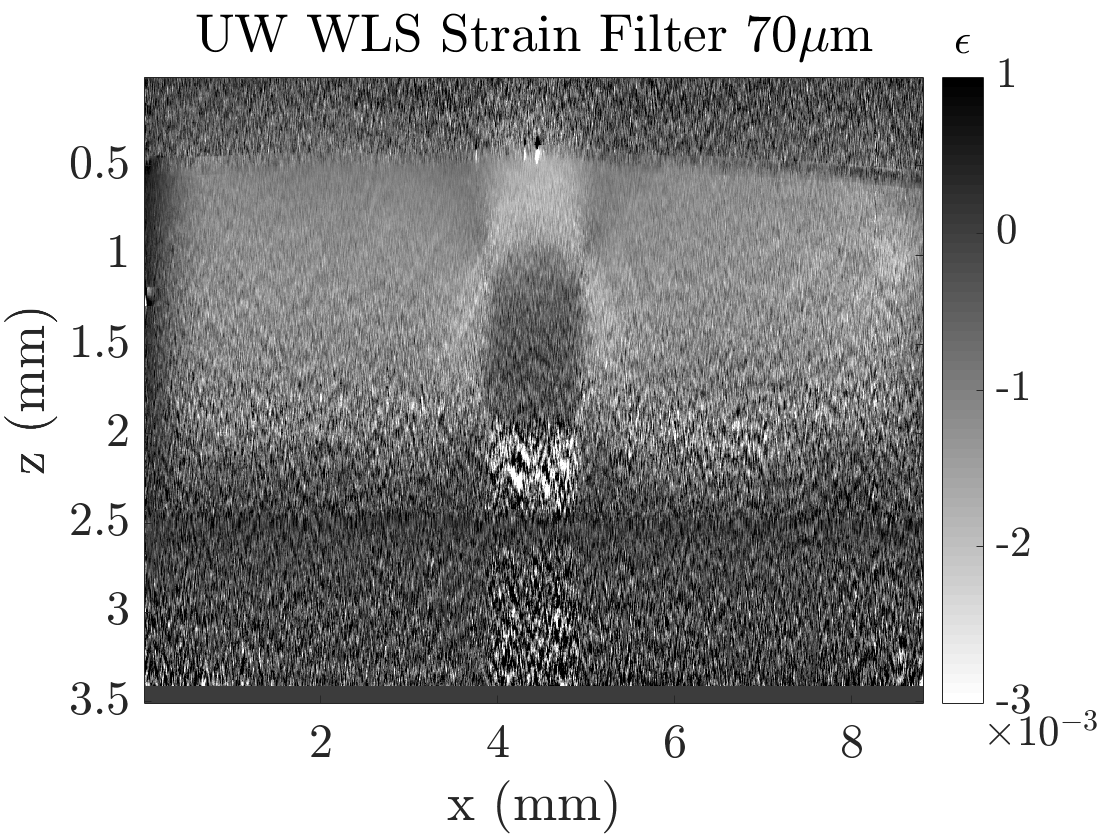
\includegraphics[width=\textwidth]{figures/wls_compare.png}
	\end{subfigure}
	\caption{\ac{uwfd} strain estimation B-scan compared with the previously standard unwrapping with \ac{uwwls}.}
	\label{wls_uwfd_compare}
\end{figure}

Taking these results in conjunction with those regarding processing time and sensitivity in the sections above, it is decided that the \ac{uwfd} strain estimation algorithm provides optimal processing speed, sensitivity, and image resolution. In particular, using a strain filter \ac{fwhm} of 40$\mu$m and a lateral smoothing filter \ac{fwhm} of 20$\mu$m should provide the best axial and image resolution, in conjunction with high sensitivity. 

The optimal strain estimation technique in this context appears to be the \ac{uwfd} algorithm, applied with lateral averaging. At a fit resolution of $40\mu m$ and a lateral smoothing resolution of $40\mu m$, all image quality parameters are improved in comparison with the previously standard \ac{uwwls} approach (\autoref{comparison_table}).

\begin{table}[h]
	\begin{tabularx}{\textwidth}{Yrrc}
		\toprule
		& \textbf{\ac{uwwls}} & \textbf{\ac{uwfd}} & \textbf{Improved?}\\
		\midrule 
		Strain Filter FWHM ($\mu$m) & 70 & 40 \\
		Lateral Smoothing Filter FWHM ($\mu$m) & 0 & 20 \\
		\midrule
		2D Processing Time (s) & & \\
		3D Processing Time (s) & 153.67 & \\
		Strain Sensitivity (m$\epsilon$) & 0.1607 & 0.1385 & 16\% \\
		Axial Image Resolution FWHM ($\mu$m) & 315.87 & 258.37 & \textbf{20\%} \\
		Lateral Image Resolution FWHM ($\mu$m) & 131.33 & 115.98 & 13\% \\
		\bottomrule
	\end{tabularx}
	\caption{Comparison of the previously standard \ac{uwwls} strain estimation technique and the optimised \ac{uwfd}.}
	\label{comparison_table}
\end{table}

\section{Future Work}

These results suggest many avenues for future work in phase-sensitive compression \ac{oce}. The process of fitting an error function to the boundaries in order to quantify the image resolution provided useful insights into the affects of averaging on different strain estimators, however the ease with which these results were obtained recommends interest in further possible application. For strain estimators that had high R-square values (such as those with lateral smoothing), and such had a robust error function fit, it may be possible to utilise an error function fitting process to routinely examine object boundaries. Examining the gradient between two objects might give insight onto what those objects actually are, particularly in the more heterogenous tissue samples. 

All strain estimators showed significant processing speed up against the \ac{uwwls}, however there is no reason to think their processing time limit has been reached. It has been discovered that \ac{gpu}s can greatly accelerate the processing of strain imaging for techniques such as ultrasound elastography that utilise speckle-tracking (rather than phase-sensitive measurement) \cite{peng_gpu-accelerated_2017}, therefore there is reason to believe this could also benefit in the phase-sensitive \ac{oce} case. Of particular benefit is the fact that all four strain estimation techniques that do not involve the volume phase unwrapping algorithm, are capable of processing individual B-scans completely independently, making it very likely that introducing parallel processing to these methods would significantly decrease the computation time. Applying filter convolutions (as in \ac{sg} filtering, and Gaussian smoothing in the \ac{fd} case) in parallel and on \ac{gpu}s could further improve the processing speed, towards intra-operative time frames, and even video-rate imaging. Before these possibilities are investigated however, the algorithms will likely need to be moved out of the Matlab interface, and applied in another language more suited to fast numerical processing.

The obvious next step for future work is to aim at translating this strain estimation algorithm into the clinic, by analysing its performance on a range of breast tissue samples. In particular, before being able to apply this technique to assess cancer margins during breast conserving surgery, diagnostic specificity and sensitivity (the ability to accurately differentiate healthy tissue from tumour) of the technique must be analysed using large case studies.

In conjunction with this, research also could be done in applying these strain estimation techniques to quantitative elastography imaging (imaging stress as well as strain), to determine which one is optimal. Measurement of a stress using a stress layer is relatively fast, and most of the computational burden falls on the strain estimation, therefore strain estimators that optimise the processing speed would benefit in this area also. 

